\chapter{Capacité du camion infinie}

Dans tout ce chapitre, on considère un graphe circulaire $G = (V,E)$ à $n$ sommets et muni d'une orientation. On suppose en outre que $p=q$, c'est-à-dire que le point de départ et d'arrivé du camion sont identiques.
\\

Par soucis de concision, nous nommerons ``algorithme dans le cas linéaire'' l'algorithme permettant d'obtenir le premier mouvement de la solution optimale et le coût d'une telle solution dans le cas où le graphe est une ligne. Cet algorithme est décrit dans l'article \cite{Benchimol2011} en section 8. On rappelle qu'un tel algorithme est linéaire en le nombre de sommet.

\section{Algorithme d'obtention de la solution optimale}
\label{Algorithme circulaire infini}

On note $S_{min}$ la meilleure solution réalisable obtenue et on l'initialise avec une solution faisant deux fois le tour du graphe (donc de coût $2\sum_{e \in E}c_e$).

La première partie de l'algorithme va comparer le coût de différentes solutions réalisables sans en calculer le premier mouvement, et une fois la solution optimale $S_{min}$ trouvée, la deuxième partie de l'algorithme donnera les mouvements successifs à faire.
\\

\textbf{Calcul du coût de la solution optimale et de ses caractéristiques :}
\begin{enumerate}
\item\label{Ze0 nul} \uline{Pour chaque $e_o \in E$}
  \begin{enumerate}
  \item Construire le graphe linéaire $\bs{G(e_0)}$ obtenu en supprimant l'arrête $e_0$ de $G$.
  \item Calculer le coût de la solution optimale $S$ à l'aide de l'algorithme dans le cas linéaire.
  \item Si $\Upsilon_{G(e_0)} < \mbox{Coût}(S_{min})$, remplacer les caractéristiques de $S_{min}$ par celles de $S$ (c'est-à-dire son coût et l'arête $e_0$).
  \end{enumerate}
\item\label{Ze0 unitaire} \uline{Pour chaque $w \in V$, pour chaque $w' \in ]w,o]_+$}
  \begin{enumerate}
  \item \uline{Premier cas : sens direct}
    \begin{enumerate}
    \item\label{Ze0 unitaire - direct} Construire le graphe linéaire $\bs{G(w,w',+)}$ obtenu en supprimant les arêtes $E\left[ \left[w',w\right]_+ \right]$ avec :
      \begin{itemize}
      \item $p=w$ et $q=w'$
      \item $x_1(w) = \sum_{v \in E\left[ \left[w',w\right]_+ \right]} x(v)$ et $y_1(w) = 0$
      \item $x_1(w') = 0$ et $y_1(w') = \sum_{v \in E\left[ \left[w',w\right]_+ \right]} y(v)$
      \end{itemize}
    \item Calculer le coût $\Upsilon_{G(w,w',+)}$ de sa solution optimale.
    \item Si $\Upsilon_{G(w,w',+)} + 3 \sum_{ v \in E\left[ \left[w',w\right]_+ \right] }c_v < \mbox{Coût}(S_{min})$, remplacer les caractéristiques de $S_{min}$ par celles de $S$ (c'est-à-dire son coût et le triplet $(w,w',+)$).
    \end{enumerate}
  \item\label{Ze0 unitaire - indirect} \uline{Deuxième cas : sens indirect}
    \begin{enumerate}
    \item Construire le graphe linéaire $\bs{G(w,w',-)}$ obtenu en supprimant les arêtes $E\left[ \left[w',w\right]_+ \right]$ avec :
      \begin{itemize}
      \item $p=w'$ et $q=w$
      \item $x_1(w') = \sum_{v \in E\left[ \left[w',w\right]_+ \right]} x(v)$ et $y_1(w') = 0$
      \item $x_1(w) = 0$ et $y_1(w) = \sum_{v \in E\left[ \left[w',w\right]_+ \right]} y(v)$
      \end{itemize}
    \item Calculer le coût $\Upsilon_{G(w,w',-)}$ de sa solution optimale.
    \item Si $\Upsilon_{G(w,w',-)} + 3 \sum_{ v \in E\left[ \left[w',w\right]_+ \right] }c_v < \mbox{Coût}(S_{min})$, remplacer les caractéristiques de $S_{min}$ par celles de $S$ (c'est-à-dire son coût et le triplet $(w,w',-)$).
    \end{enumerate}
  \end{enumerate}
\end{enumerate}

\textbf{Calcul de la solution optimale :}
\begin{enumerate}
\item\label{Calcul mvt - Ze0 nul} Si $S_{min}$ est caractérisée par une arête $e_0$.
  \begin{enumerate}
  \item Construire le graphe linéaire $\bs{G(e_0)}$.
  \item Calculer les mouvements successifs de la solution optimale à l'aide de l'algorithme dans le cas linéaire sur le graphe $\bs{G(e_0)}$.
  \end{enumerate}
\item\label{Calcul mvt - Ze0 unitaire - direct} Si $S_{min}$ est caractérisée par un triplet $(w,w',+)$.
  \begin{enumerate}
  \item démarrer en $p$.
  \item aller jusqu'à $w'$ dans le sens négatif.
  \item aller jusqu'à $w$ dans le sens positif en ramassant tous les vélos présents sur le chemin.
  \item Construire le graphe linéaire $\bs{G(w,w',+)}$.
  \item Calculer les mouvements successifs de la solution optimale à l'aide de l'algorithme dans le cas linéaire sur le graphe $\bs{G(w,w',+)}$.
  \item aller jusqu'à $w$ dans le sens positif en équilibrant toutes les stations parcourues.
  \item revenir en $p$ dans le sens négatif.
  \end{enumerate}
\item\label{Calcul mvt - Ze0 unitaire - indirect} Si $S_{min}$ est caractérisée par un triplet $(w,w',-)$.
  \begin{enumerate}
  \item démarrer en $p$.
  \item aller jusqu'à $w$ dans le sens positif.
  \item aller jusqu'à $w'$ dans le sens négatif en ramassant tous les vélos présents sur le chemin.
  \item Construire le graphe linéaire $\bs{G(w,w',-)}$.
  \item Calculer les mouvements successifs de la solution optimale à l'aide de l'algorithme dans le cas linéaire sur le graphe $\bs{G(w,w',-)}$.
  \item aller jusqu'à $w'$ dans le sens négatif en équilibrant toutes les stations parcourues.
  \item revenir en $p$ dans le sens positif.
  \end{enumerate}
\end{enumerate}


\begin{thm} \label{thm: optimalité algo infini}
La solution $S_{min}$ retournée à la fin de l'algorithme précédent est une solution réalisable optimale et la complexité de l'algorithme est cubique en le nombre de sommets du graphe.

De plus, le coût de la solution optimale est donnée par
$$
\Upsilon_{G} = \min
\left(
  \min_{e \in E} \Upsilon_{G(e)}\,,\,
  \min_{w \in V, w' \in ]w,o]}
  \left(
    3 \sum_{ v \in E\left[ \left[w',w\right]_+ \right] }c_v + \min \left( \Upsilon_{G(w,w',+)} \,,\, \Upsilon_{G(w,w',-)} \right)
  \right)
\right).
$$
\end{thm}

La suite de ce chapitre va permettre de montrer ce théorème.

\section{Conditions nécessaires pour qu'une solution réalisable soit optimale}

\subsection{Borne supérieure du coût de la solution optimale}

\begin{lem}\label{capacite infinie - borne sup cout}
\emph{Borne supérieure du coût de la solution optimale}\\
Si la capacité $C$ du camion est infine et si $p=q$, alors le coût d'une solution optimale du SSBP est strictement inférieur $\displaystyle 2\sum_{e \in E}c_e$.
\end{lem}

\begin{proof}
Il suffit d'aller de $p$ à $p-1$ dans le sens positif en prenant tous les vélos sur chaque station (y compris en $p$). Tous les vélos du modèle sont alors dans le camion et toutes les stations sont vides. Puis il suffit de revenir de $p-1$ à $p$ dans le sens négatif en posant sur chaque station le nombre de vélo nécessaire pour l'équilibrer.
\end{proof}

En pratique, une capacité infinie signifie que la capacité du camion est supérieure au nombre total de vélos sur le graphe.

\subsection{Parité des $z_e$}

\begin{prop}\label{parité des Ze}
Soit $G=(V,E)$ un graphe connexe. Si $p=q$, alors tous les $z_e$ ont la même parité.
\end{prop}

\begin{proof}
Comme $p=q$, la condition d'Euler est également vérifiée pour $p$. Donc $z(\delta(v))$ est paire pour tout $v \in V$.\\
Soit $e \in E$. Selon la condition d'Euler, $z(\{e, e+1\}) = z_e + z_{e+1}$ est paire. Donc $z_e$ et $z_{e+1}$ ont la même parité. Par une récurrence immédiate, tous les $z_e$ ont la même parité.
\end{proof}

\subsection{Restriction du nombre de passages sur une arête particulière}

\begin{prop}
On suppose que la capacité $C$ du camion est infine et que $p=q$. Soit $S$ une solution optimale du SSBP. Alors il existe une arrête $e_0 \in E$ tel que le camion passe au plus une fois par $e_0$.
\end{prop}

\begin{proof}
Par l'absurde, on suppose que pour tout $e \in E$, le camion passe au moins deux fois sur $e$. Alors le coût de la solution optimale est supérieur à $2\sum_{e \in E}c_e$ ce qui contredit le lemme \ref{capacite infinie - borne sup cout}.
\end{proof}

De cette proposition, on en déduit qu'il suffit de distinguer deux cas :
\begin{itemize}
\item \uline{il existe $e_0 \in E$ tel que le camion ne passe pas par $e_0$.}\\
Dans la partie \ref{Ze0 nul} de l'agorithme, on trouve pour chaque $e_0$ enlevé une solution optimale sous contrainte $z_{e_0} = 0$ et on garde la meilleure.
\item \uline{le camion passe au moins une fois par tous les sommets et il existe $e_0 \in E$ tel que le camion passe exactement une fois par $e_0$.}\\
On démontrera que dans la partie \ref{Ze0 unitaire}, on trouve pour chaque $e_0$ une solution optimale sous contrainte $z_{e_0} = 1$ et on garde la meilleure.
\end{itemize}

\subsection{Restriction du nombre de passages sur l'ensemble des arêtes}

\begin{prop}\label{Ze inf 3 - lineaire}
Soit $G=(V,E)$ un graphe linéaire. On suppose que la capacité $C$ du camion est infine et que $p$ et $q$ sont des extrémités du grapghe. Alors il existe une solution réalisable optimale telle que : pour toute arête $e \in E$, le camion passe au plus trois fois sur $e$.
\end{prop}

\begin{proof}
Les auteurs de l'article \cite{Benchimol2011} ont donné un algorithme et une formule pour calculer les $z_e$ d'une solution optimale particulière. Pour $e \in E$
\begin{gather*}
  z_e = \mbox{max}
  \bigg(
    \underbrace{ 2 \left\lceil \frac{x(U_e)-y(U_e)}{C} \right\rceil\ }_{\displaystyle \le 2 \mbox{ (car } C\mbox{ est infinie)} } +
    \underbrace{ \eta(p,q,U_e) }_{\displaystyle \le 1}\,,\,
    \underbrace{ \mu(p,q,U,\bs{x},\bs{y}) }_{\displaystyle \le 2}
  \bigg)
  \le 3
\end{gather*}
\end{proof}

\begin{lem}\label{Ze inf 3 - circulaire}
Soit $G=(V,E)$ un graphe circulaire. On suppose que la capacité $C$ du camion est infine et que $p=q$. Alors il existe une solution réalisable optimale telle que : pour toute arête $e \in E$, le camion passe au plus trois fois sur $e$.
\end{lem}

\begin{figure}[ht]
  \centering
  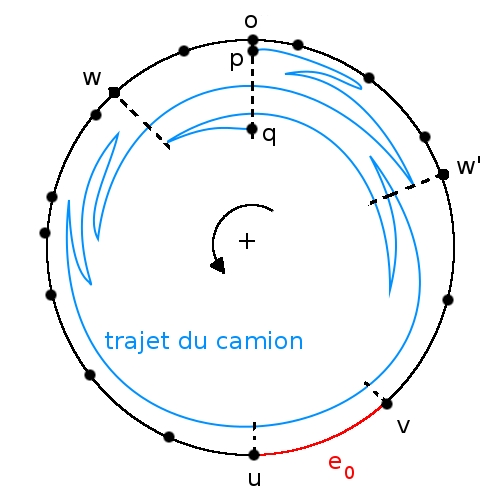
\includegraphics[scale=0.5]{GrapheCirculaire_PreuveZeInf3.jpg}
  \caption{Notations utilisées dans le cas du graphe circulaire avec une capacité infinie}
  \label{Notation graphe circulaire preuve Ze inf 3}
\end{figure}

\begin{proof}\uline{$1^{\mbox{er}}$ cas} : \uline{il existe $e_0 \in E$ tel que le camion ne passe pas par $e_0$.}

Le calcul de la solution optimale se ramène au cas du graphe linéaire $G(e_0)$ obtenu en supprimant l'arête $e_0$ du graphe $G$. Selon la proposition \ref{Ze inf 3 - lineaire}, la solution optimale passe au plus trois fois par chaque arête de $G(e_0)$ donc de $G$.
\\

\uline{$2^{\mbox{ème}}$ cas} : \uline{le camion passe au moins une fois par tous les sommets et il existe $e_0 \in E$ tel que le camion passe exactement une fois par $e_0$.}

Soit $S$ une solution optimale sous contrainte $z_{e_0} = 1$. On note $o=p=q$ le point de départ et d'arrivée du camion. Quitte à changer l'orientation du graphe, on peut supposer que $e_0$ est parcourue dans le sens positif. et on note $u$ le sommet par lequel on entre sur $e_0$ et $v$ le sommet par lequel on sort de $e_0$. (cf figure \ref{Notation graphe circulaire preuve Ze inf 3} pour une synthèse des notations.)

Soit $w$ le sommet sur la portion $[o,u]_+$ le plus proche de $u$ et qui soit atteint par le camion après le parcours de $e_0$. Soit $w'$ le sommet sur la portion $[v,o]_+$ le plus proche de $v$ et qui soit atteint par le camion avant le parcours de $e_0$. Ces deux sommets sont bien définis car $o$ est atteint avant et après le passage sur $e_0$.

Alors, on peut toujours construire une solution optimale $S'$ comme suit :
\begin{enumerate}
\item\label{NewS1} démarrer en $o$.
\item\label{NewS2} aller jusqu'à $w'$ dans le sens négatif.
\item\label{NewS3} aller jusqu'à $w$ dans le sens positif en ramassant tous les vélos présents sur le chemin.
\item\label{NewS4} équilibrer la portion $[w,w']_+$ à l'aide de l'algorithme du cas linéaire sur le graphe $G(w,w',+)$ obtenu à partir de $G$ en supprimant les arêtes $E\left[[w,w']_+\right]$ et tel que :
  \begin{itemize}
  \item $p=w$ et $q=w'$
  \item $\displaystyle x_1(w) = \sum_{v \in E\left[ \left[w',w\right]_+ \right]} x(v)$ et $y_1(w) = 0$
  \item $x_1(w') = 0$ et $\displaystyle y_1(w') = \sum_{v \in E\left[ \left[w',w\right]_+ \right]} y(v)$
  \end{itemize}
\item\label{NewS5} aller jusqu'à $w$ dans le sens positif en équilibrant toutes les stations parcourues.
\item\label{NewS6} revenir en $o$ dans le sens négatif.
\end{enumerate}
Il reste à démontrer que $S'$ équilibre bien le graphe et que $\mbox{Coût}(S') \le \mbox{Coût}(S)$.
\\

\uline{Montrons que $S'$ équilibre bien le graphe.}

\`A l'étape \ref{NewS4}, tous les vélos sont présent dans la portion $[w,w']_+$. La résolution à l'aide de l'algorithme du cas linéaire sur le graphe extrait décrit ci-dessus permet donc d'équilibrer la portion de graphe avec au plus trois passages sur chaque arête de $E\left[[w,w']_+\right]$ (cf Proposition \ref{Ze inf 3 - lineaire}).

\`A la fin de l'étape \ref{NewS4}, les stations de la portion $]w,w'[_+$ sont équilibrées et celles de la portion $[w',w]_+$ sont vides et tous les vélos nécessaires pour l'équilibrer sont sur $w'$. L'étape \ref{NewS5} permet donc bien d'équilibrer les stations de $[w',w]_+$ et l'étape \ref{NewS6} de revenir en $o$.
\\

\uline{Montrons que $\mbox{Coût}(S') \le \mbox{Coût}(S)$.}

Par construction de $w$ et $w'$ la solution $S$ passait au moins trois fois par chaque arête de $[w',w]_+$. Or $S'$ passe exactement trois fois par chaque arête de $[w',w]_+$. Donc $z_e' \le z_e$ pour tout $e \in E\left[ \left[w',w\right]_+\right]$.

On s'intéresse à la solution $S$. On suppose qu'une fois le camion rentré dans $]w,w'[_+$, il retourne dans $[w',w]_+$ en entrant par $w$.\\
- S'il revenait pour prendre des vélos, il aurait pu le faire avant d'entrer dans $]w,w'[_+$.\\
- S'il venait pour poser des vélos, il pourrait le faire après être sorti de $]w,w'[_+$.

On suppose qu'une fois le camion sorti de $]w,w'[_+$, il retourne dans $[w',w]_+$ en entrant par $w'$.\\
- S'il revenait pour prendre des vélos, il aurait pu le faire avant de sortir de $]w,w'[_+$.\\
- S'il venait pour poser des vélos, il aurait pu les prendre avant d'entrer dans $]w,w'[_+$ et les poser une fois à l'intérieur de $]w,w'[_+$.

On en déduit que la solution $S$ équilibre la portion $]w,w'[_+$ comme s'il s'agissait du graphe linéaire $G(w,w',+)$ décrit ci-dessus.
Donc le coût pour équilibrer $]w,w'[_+$ dans $S$ et dans $S'$ est le même.

On en déduit que $\mbox{Coût}(S') \le \mbox{Coût}(S)$ et donc que $S'$ est optimale et réalisable.

Par construction, $S'$ passe au plus trois fois par chaque arête, ce qui conclut la démonstration.
\end{proof}

\section{Preuve de l'optimalité de l'algorithme}

Comme le calcul du coût d'une solution optimale dans le cas d'un graphe linéaire est linéaire en le nombre de sommet, il est évident que l'algorithme décrit en section \ref{Algorithme circulaire infini} est cubique en le nombre de sommet $n$ du graphe $G$.

De plus, il est évident que :
\begin{itemize}
\item $\min_{e \in E} \Upsilon_{G(e)}$ donne le coût de la meilleure solution retourné dans la partie \ref{Calcul mvt - Ze0 nul}.
\item $\min_{w \in V, w' \in ]w,o]} \left(3 \sum_{ v \in E\left[ \left[w',w\right]_+ \right] }c_v + \Upsilon_{G(w,w',+)}\right)$ donne le coût de la meilleure solution retourné dans la partie \ref{Calcul mvt - Ze0 unitaire - direct}.
\item $\min_{w \in V, w' \in ]w,o]} \left(3 \sum_{ v \in E\left[ \left[w',w\right]_+ \right] }c_v + \Upsilon_{G(w,w',-)}\right)$ donne le coût de la meilleure solution retourné dans la partie \ref{Calcul mvt - Ze0 unitaire - indirect}.
\end{itemize}
Donc la formule donnée dans le théorème \ref{thm: optimalité algo infini} donne bien le coût de la meilleure solution retournée par l'algorithme.

Il reste à montrer que l'algorithme renvoie bien une solution optimale.